% Appendix B

\chapter{Notation} % Main appendix title

\label{AppendixB} % For referencing this appendix elsewhere, use \ref{AppendixA}
\begin{figure}[th]
\centering
\includegraphics{Figures/outMoneyAmerP.png}
\decoRule
\caption[MLPs Performance for Out-of-money datasets on American Put]{MLPs Performance for Out-of-money datasets on American Put, where the targets are from the binomial model}
\label{fig:MLPsAmerPOutMoney}
\end{figure}

\begin{figure}[th]
\centering
\includegraphics{Figures/longTAmerP.png}
\decoRule
\caption[MLPs Performance for Out-of-money datasets on American Put]{MLPs Performance for Out-of-money datasets on American Put, where the targets are from the binomial model}
\label{fig:MLPsAmerPLongT}
\end{figure}

\begin{figure}[th]
\centering
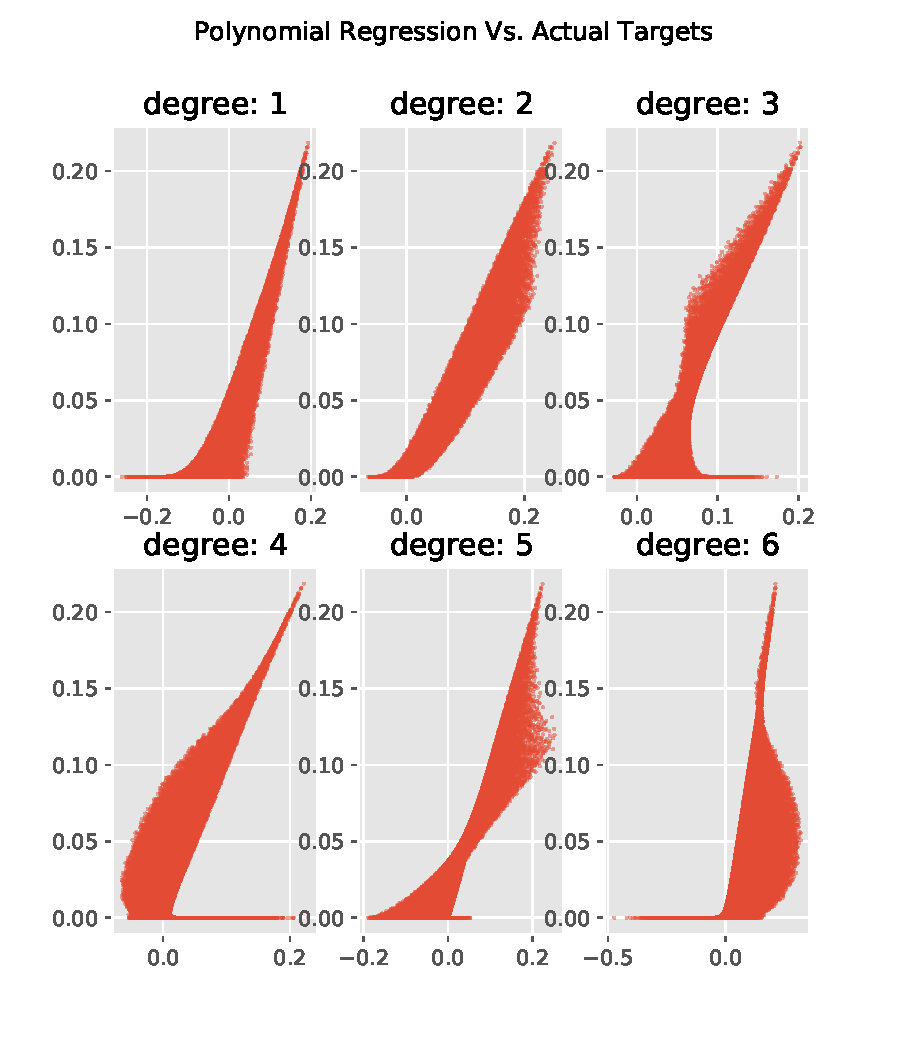
\includegraphics{Figures/polynomialOutMoneyEuroC.png}
\decoRule
\caption[Polynomial Regression Performance on out-of-money dataset European Call]{Polynomial Regression Performance on out of money dataset on european call}
\label{fig:MLPsEuroCOutOfMoney}
\end{figure}



\begin{figure}[th]
\centering
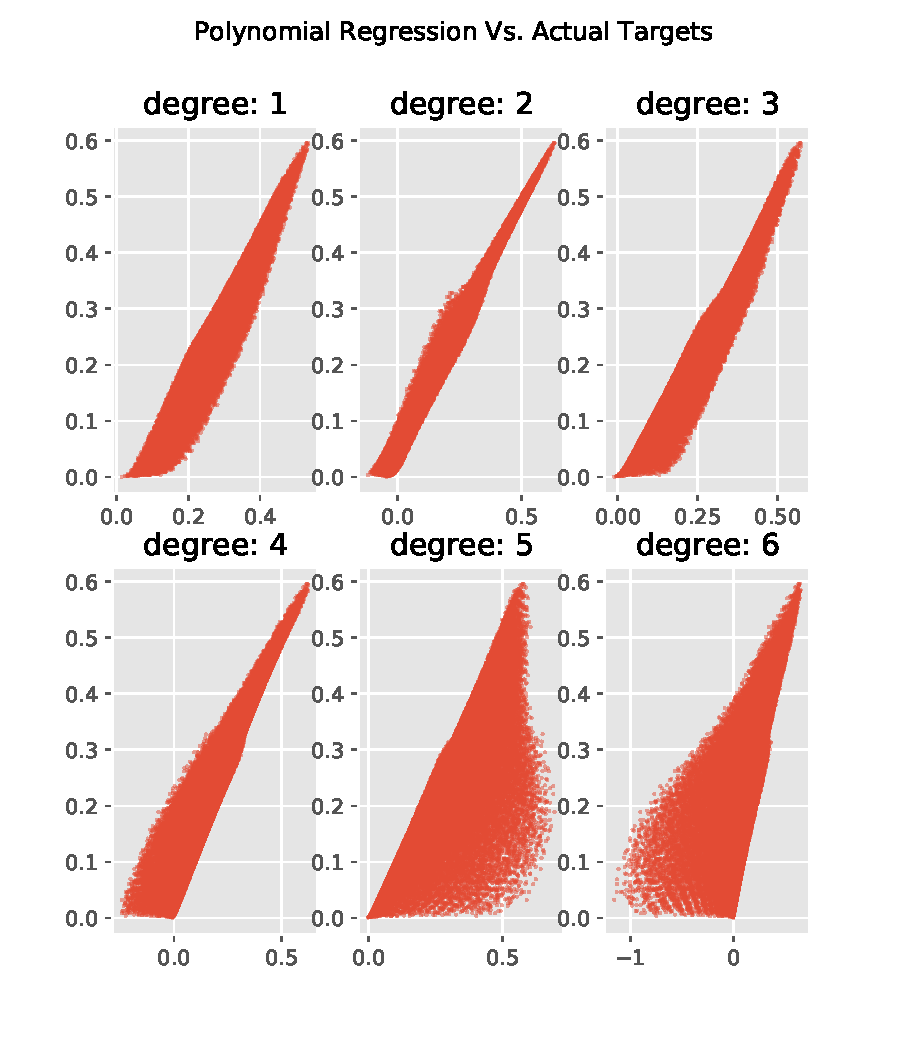
\includegraphics{Figures/polynomialLongTEuroC.png}
\decoRule
\caption[Polynomial Regression Performance on long maturity dataset European Call]{Polynomial Regression Performance on long maturity dataset on european call}
\label{fig:MLPsEuroCLongMaturity}
\end{figure}


We choose grid search with the cartesian product, where b denote the batchsize.
$$\eta \times b = \{(\eta,b) : \eta \in \{0.0001, 0.001, 0.01 \} \ and \ b \in \{8, 256, 1024\} \}$$
\begin{table}[th]
\caption{Hyperparameter tuning of learning rate and batchsize for american put minimum two assets for the interested reader see the tensorboard (link \href{https://tensorboard.dev/experiment/A3oOYhPiQoiDZgsNXVazPg/\#scalars}{tensorboard 3})}
\label{tab:hyperAmerMin2}
\centering
\begin{tabular}{l l l l }
\toprule
\textbf{Model} & \textbf{lr} & \textbf{Batch Size} & \textbf{Loss} \\
\midrule
MLPs & 0.00010000 & 1024 & 5.7394\\
&	0.00010000 & 256 & 2.1029\\
&	0.00010000 & 8 & 0.92074\\
&	0.00100000 & 1024 & 6.3428\\
& 	0.00100000 & 256 & 1.2985 \\
& 	0.00100000 & 8 & 0.070993\\
&	0.01000000 & 1024 & 6.1258 \\
& 	0.01000000 & 256 & 1.4931\\
& 	0.01000000 & 8 & 8.1098\\
\bottomrule\\
\end{tabular}
\end{table}

\begin{table}[th]
\caption{Hyperparameter tuning of dataset size and batchsize for american put minimum two assets for the interested reader see the tensorboard (link \href{https://tensorboard.dev/experiment/r6LTlLGaTMCXrKOJpl4Qmg/\#scalars}{tensorboard 4})}
\label{tab:hyperAmerMin3}
\centering
\begin{tabular}{l l l l }
\toprule
\textbf{Model} & \textbf{Dataset Size} & \textbf{Batch Size} & \textbf{Loss} \\
\midrule
MLPS & 800 & 8 & 7.6495\\
&	800 & 64 & 36.535\\
&	80K & 8 & 0.082552\\
&	80K & 64 & 0.091618 \\
& 	240K & 8 & 0.073089 \\
& 	240K & 64 & 0.091618 \\
\bottomrule\\
\end{tabular}
\end{table}


From the above table we see that the best configuration on this run is for $\eta=0.001$ and $b=8$. LIke for the european option we will investigate if the dataset size matter for the loss of our model. We choose to the learning $\eta=0.001$ by above test and we vary b in the set $b=\{8, 64\}$, beacuse we might suspect a higger batchsize is better for a bigger dataset.



From above table \ref{tab:hyperAmerMin2} the training error improves with bigger dataset, hence we choose the dataset with 300.000 samples, where from the training set a validation set of size 60.000 is subsampled. The above study is never complete, but we have seem with grid search the optimal choice for the learning rate, batch size and datasize. Below we will try a different model than MLPs to see if we really need deep learning for this method. 


\begin{table}[th]
\caption{Hyperparameter tuning of dataset size and batchsize for american put minimum two assets for the interested reader see the tensorboard}
\label{tab:fullhyperAmerMin4}
\centering
\begin{tabular}{|l|l|l|l|}
\toprule
\textbf{Model} & \textbf{Dataset Size} & \textbf{Batch Size} & \textbf{Loss} \\
\midrule
300K    & 0.0001 & 8     & 0.015130897983909 \\ \hline
300K    & 0.001  & 64    & 0.035523075610399 \\ \hline
100K    & 0.0001 & 8     & 0.064886227250099 \\ \hline
100K    & 0.001  & 8     & 0.072143875062466 \\ \hline
300K    & 0.0001 & 64    & 0.075988814234734 \\ \hline
300K    & 0.001  & 8     & 0.104622706770897 \\ \hline
300K    & 0.01   & 256   & 0.480043411254883 \\ \hline
300K    & 0.0001 & 256   & 1.04093873500824  \\ \hline
300K    & 0.001  & 256   & 1.06809389591217  \\ \hline
300K    & 0.001  & 512   & 1.08942472934723  \\ \hline
100K    & 0.001  & 64    & 1.18230485916138  \\ \hline
300K    & 0.001  & 1024  & 1.30065310001373  \\ \hline
300K    & 0.01   & 512   & 1.45135951042175  \\ \hline
100K    & 0.01   & 256   & 1.52623510360718  \\ \hline
300K    & 0.01   & 64    & 1.75954759120941  \\ \hline
300K    & 0.01   & 1024  & 1.92213356494904  \\ \hline
100K    & 0.01   & 512   & 2.01193928718567  \\ \hline
100K    & 0.01   & 64    & 2.02969717979431  \\ \hline
300K    & 0.0001 & 1024  & 5.72439670562744  \\ \hline
300K    & 0.0001 & 512   & 5.72847843170166  \\ \hline
100K    & 0.0001 & 256   & 5.76278400421143  \\ \hline
100K    & 0.0001 & 512   & 5.77397203445435  \\ \hline
100K    & 0.0001 & 64    & 5.80239868164063  \\ \hline
100K    & 0.0001 & 1024  & 5.90070772171021  \\ \hline
100K    & 0.001  & 256   & 6.29003953933716  \\ \hline
100K    & 0.001  & 512   & 6.52896738052368  \\ \hline
100K    & 0.001  & 1024  & 6.56187915802002  \\ \hline
1K      & 0.001  & 8     & 7.5845251083374   \\ \hline
100K    & 0.01   & 8     & 8.07239627838135  \\ \hline
1K      & 0.01   & 8     & 11.7414264678955  \\ \hline
100K    & 0.01   & 1024  & 13.4287099838257  \\ \hline
1K      & 0.01   & 64    & 14.1254253387451  \\ \hline
1K      & 0.0001 & 8     & 24.0087566375732  \\ \hline
1K      & 0.001  & 64    & 27.0112972259521  \\ \hline
1K      & 0.01   & 512   & 40.0226554870605  \\ \hline
1K      & 0.001  & 512   & 44.841724395752   \\ \hline
1K      & 0.01   & 256   & 45.8363571166992  \\ \hline
1K      & 0.01   & 1024  & 49.3933792114258  \\ \hline
1K      & 0.0001 & 64    & 51.3070755004883  \\ \hline
1K      & 0.001  & 256   & 52.8623466491699  \\ \hline
1K      & 0.0001 & 512   & 87.4313125610352  \\ \hline
1K      & 0.0001 & 256   & 89.8093795776367  \\ \hline
1K      & 0.0001 & 1024  & 90.8342361450195  \\ \hline
\bottomrule\\
\end{tabular}
\end{table}

\begin{figure}[th]
\centering
\includegraphics[width=\textwidth]{Figures/euroTestDataset.png}
\decoRule
\caption[Effect of dataset size]{MLPs regression training for european call, where the plot shows the effect of gather more data on training and validation loss, where the x-axis is number of epoch-1 and y-axis is the loss for the training and validation loop. The orange line with the largest error is for 100 datapoints, the grey line for 1000 datapoints, the green line 10K datapoints, the three last lines blends together where it is for 100K,300K and 1M datapoints. More can be seem at tensorboard (link \href{https://tensorboard.dev/experiment/JURHMdo6Ra6MRW5XnlYwkg/\#scalars&run=EuroCall\%2FEuroMLP1K\&\_smoothingWeight=0\&runSelectionState=eyJFdXJvQ2FsbC9FdXJvTUxQMTAwIjp0cnVlLCJFdXJvQ2FsbC9FdXJvTUxQMTAwLzE2MDE5MjcyNTMuOTkyMTYxMyI6dHJ1ZSwiRXVyb0NhbGwvRXVyb01MUDEwMC8xNjAxOTI3MjU0LjAwODY1NTUiOnRydWUsIkV1cm9DYWxsL0V1cm9NTFAxMDAvMTYwMTkyNzI1NC4wMjYzMTA3Ijp0cnVlLCJFdXJvQ2FsbC9FdXJvTUxQMTAwLzE2MDE5MjcyNTQuMDQzODcyIjp0cnVlLCJFdXJvQ2FsbC9FdXJvTUxQMTAwLzE2MDE5MjcyNTQuMDU3NjkwNCI6dHJ1ZSwiRXVyb0NhbGwvRXVyb01MUDEwMC8xNjAxOTI3MjU0LjA2NzcyOTIiOnRydWUsIkV1cm9DYWxsL0V1cm9NTFAxMDAvMTYwMTkyNzI1NC4wODIzMDczIjp0cnVlLCJFdXJvQ2FsbC9FdXJvTUxQMTAwLzE2MDE5MjcyNTQuMDg5ODkzNiI6dHJ1ZSwiRXVyb0NhbGwvRXVyb01MUDEwMC8xNjAxOTI3MjU0LjEwMDA5ODQiOnRydWUsIkV1cm9DYWxsL0V1cm9NTFAxMDAvMTYwMTkyNzI1NC4xMTk4NSI6dHJ1ZSwiRXVyb0NhbGwvRXVyb01MUDEwMEsiOnRydWUsIkV1cm9DYWxsL0V1cm9NTFAxMEsiOnRydWUsIkV1cm9DYWxsL0V1cm9NTFAxSyI6dHJ1ZSwiRXVyb0NhbGwvRXVyb01MUDFNIjp0cnVlLCJFdXJvQ2FsbC9FdXJvTUxQMU0vMTYwMTkyNzQ4NC44MzczMjQ5Ijp0cnVlLCJFdXJvQ2FsbC9FdXJvTUxQMU0vMTYwMTkyNzUzMS42OTg0MjciOnRydWUsIkV1cm9DYWxsL0V1cm9NTFAxTS8xNjAxOTI3NTgwLjYxOTQwODQiOnRydWUsIkV1cm9DYWxsL0V1cm9NTFAxTS8xNjAxOTI3NjMxLjEwNjM5ODgiOnRydWUsIkV1cm9DYWxsL0V1cm9NTFAxTS8xNjAxOTI3Njc3LjEzMTg4MjIiOnRydWUsIkV1cm9DYWxsL0V1cm9NTFAxTS8xNjAxOTI3NzIyLjg2Nzk2ODMiOnRydWUsIkV1cm9DYWxsL0V1cm9NTFAxTS8xNjAxOTI3NzY4LjY2MDgwODYiOnRydWUsIkV1cm9DYWxsL0V1cm9NTFAxTS8xNjAxOTI3ODE0LjA0NjU0NiI6dHJ1ZSwiRXVyb0NhbGwvRXVyb01MUDFNLzE2MDE5Mjc4NTkuMDAzNzc5Ijp0cnVlLCJFdXJvQ2FsbC9FdXJvTUxQMU0vMTYwMTkyNzkwNC4xODYyODciOnRydWUsIkV1cm9DYWxsL0V1cm9NTFAzMDBLIjp0cnVlfQ\%3D\%3D}{tensorboard 5})}
\label{fig:dataComparisonEuroMLP}
\end{figure}


Long maurity polynomial regression:
['MSE test 0.002662', 'MSE test 0.001196', 'MSE test 0.001654', 'MSE test 0.003956', 'MSE test 0.012255', 'MSE test 0.043361']
['RMSE test 0.051593', 'RMSE test 0.034577', 'RMSE test 0.040666', 'RMSE test 0.062894', 'RMSE test 0.110702', 'RMSE test 0.208233']
['MAE test 0.041232', 'MAE test 0.026287', 'MAE test 0.028371', 'MAE test 0.039932', 'MAE test 0.064402', 'MAE test 0.111190']
['R2 test 0.818143', 'R2 test 0.918316', 'R2 test 0.887014', 'R2 test 0.729744', 'R2 test 0.162742', 'R2 test -1.962442']

In-sample polynomial regression:
['MSE test 0.000636', 'MSE test 0.000069', 'MSE test 0.000013', 'MSE test 0.000004', 'MSE test 0.000002', 'MSE test 0.000001']
['RMSE test 0.025212', 'RMSE test 0.008316', 'RMSE test 0.003624', 'RMSE test 0.002052', 'RMSE test 0.001414', 'RMSE test 0.000958']
['MAE test 0.018326', 'MAE test 0.006141', 'MAE test 0.002561', 'MAE test 0.001280', 'MAE test 0.000867', 'MAE test 0.000591']
['R2 test 0.936628', 'R2 test 0.993105', 'R2 test 0.998691', 'R2 test 0.999580', 'R2 test 0.999801', 'R2 test 0.999909']

Out-of-money maurity polynomial regression:
['MSE test 0.005772', 'MSE test 0.000767', 'MSE test 0.000839', 'MSE test 0.000944', 'MSE test 0.001812', 'MSE test 0.004423']
['RMSE test 0.075973', 'RMSE test 0.027694', 'RMSE test 0.028960', 'RMSE test 0.030724', 'RMSE test 0.042568', 'RMSE test 0.066506']
['MAE test 0.060936', 'MAE test 0.022203', 'MAE test 0.020288', 'MAE test 0.020542', 'MAE test 0.027125', 'MAE test 0.041315']
['R2 test -2.377251', 'R2 test 0.551246', 'R2 test 0.509280', 'R2 test 0.447668', 'R2 test -0.060261', 'R2 test -1.588030']


\begin{figure}[th]
\centering
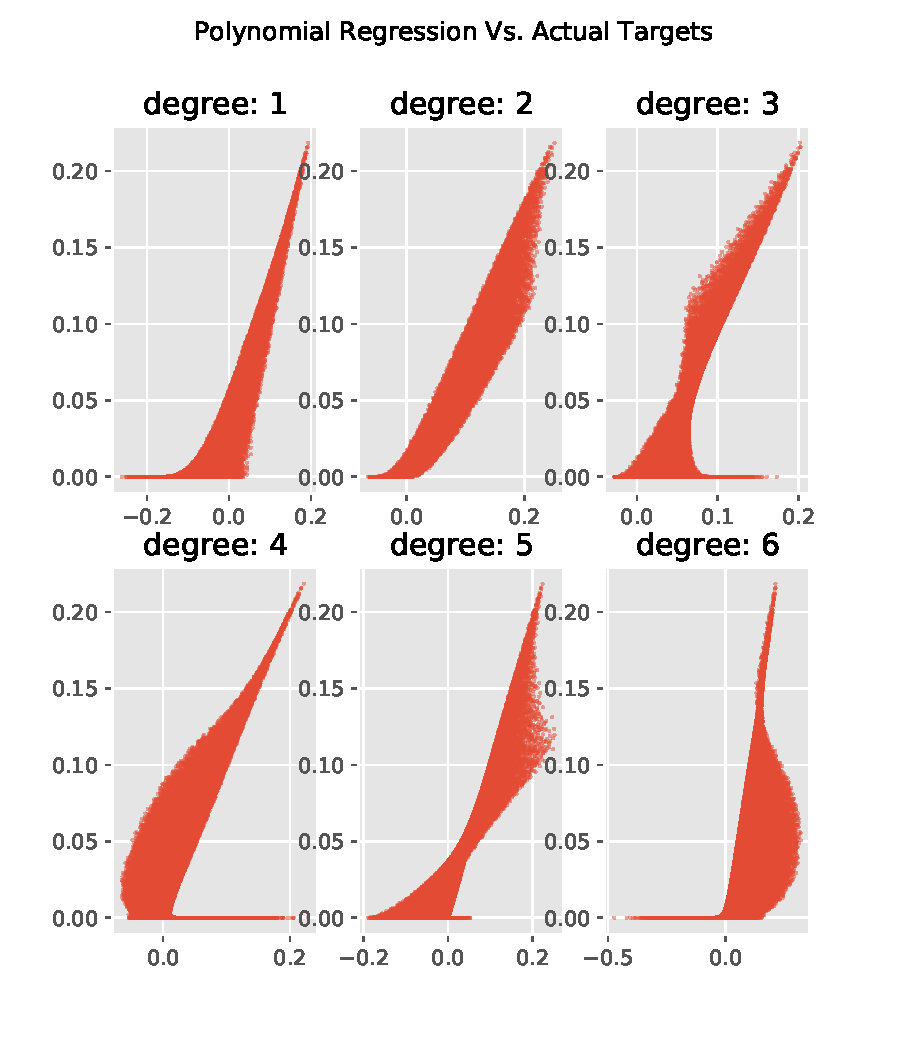
\includegraphics{Figures/polynomialOutMoneyEuroC.png}
\decoRule
\caption[Polynomial Regression Predictions Vs. Actual Prices]{Predicted price based on polynomial regression of varying degree}
\label{fig:PolynomialOutMoneyEuroC}
\end{figure}

\begin{figure}[th]
\centering
\includegraphics{Figures/PredictionOutMoneyEuroC.png}
\decoRule
\caption[MLPs Predictions Vs. Actual Prices]{Predicted price based on MLPs model}
\label{fig:MLPsOutMoneyEuroC}
\end{figure}

\begin{figure}[th]
\centering
\includegraphics{Figures/longTAmerMinP.png}
\decoRule
\caption[MLPs Performance on long maturity dataset on American bivariate contingent claim]{MLPs Performance on long maturity dataset on American put on minimum of two stocks}
\label{fig:MLPsEuroC}
\end{figure}


\begin{figure}[th]
\centering
\includegraphics{Figures/inMoneyAmerMinP.png}
\decoRule
\caption[MLPs Performance on long maturity dataset on American bivariate contingent claim]{MLPs Performance on long maturity dataset on American put on minimum of two stocks}
\label{fig:MLPsEuroC}
\end{figure}